\documentclass[10pt]{exam}
\usepackage[hon]{template-for-exam}
\usepackage{tikz}
\usetikzlibrary{shadings,decorations.pathmorphing,arrows.meta,patterns}

\title{Elastic Collisions}
\author{Rohrbach}
\date{\today}

\begin{document}
\maketitle




\noindent
Two balls shown below ($m_A=0.15$ kg and $m_B=0.18$ kg) are constrained to move in one dimension.  If they undergo a totally elastic collision, what is the final velocity of each ball?

\vspace{2em}

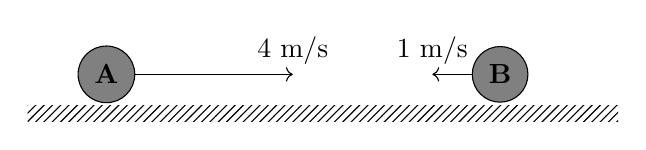
\begin{tikzpicture}
  \node[circle, fill=gray, draw=black] at (0,0) (A) {\bf A};
  \node[circle, fill=gray, draw=black] at (5,0) (B) {\bf B};
  \draw[->] (A.east) -- ++(2,0) node[above] {4 m/s};
  \draw[->] (B.west) -- ++(-.5,0) node[above] {1 m/s};
  \fill[pattern=north east lines]
    (-1,-0.4) rectangle ++(7.5,-0.2);
\end{tikzpicture}

\vs

\noindent
What if the collision is totally inelastic?

\vs

\end{document}